\documentclass[../psets.tex]{subfiles}

\pagestyle{main}
\renewcommand{\leftmark}{Problem Set 3}

\begin{document}




\begin{enumerate}[label={\Roman*)}]
    \item \marginnote{2/4:}Ammonia undergoes a facile inversion ("umbrella flip") as shown below. The activation barrier for inversion is low ($\Delta G^\ddagger\sim\SI{5}{kcal\per\mole}$), and the transition state for this motion is planar \ce{NH3}. Note that the relevant valence shell IP's are $\ce{N}_{2s}=\SI{-26.0}{eV}$, $\ce{N}_{2p}=\SI{-13.4}{eV}$, and $\ce{H}_{1s}=\SI{-13.6}{eV}$.
    \begin{center}
        \schemestart
            \chemfig{\charge{90=\:}{N}(-[:-30]H)(>:[:-150]H)(<[:-110]H)}\arrow{<=>}
            \chemleft{[}
                \chemfig{\charge{180=\:}{N}(-H)(>:[:150]H)(<[:-150]H)}
            \chemright{]^{\ddagger}}\arrow{<=>}
            \chemfig{\charge{-90=\:}{N}(-[:30]H)(>:[:150]H)(<[:110]H)}
        \schemestop
    \end{center}
    \begin{enumerate}[label={\alph*)}]
        \item Construct an MO diagram for \emph{planar} \ce{NH3}.
        \begin{proof}[Answer]
            Point group: $D_{3h}$\par
            Basis functions: all three \ce{H} orbitals, \ce{N_{$2s$}}, \ce{N_{$2p_x$}}, \ce{N_{$2p_y$}}, and \ce{N_{$2p_z$}}.\par
            Apply operations, generate reducible representations, and reduce to irreducible representations:
            \begin{align*}
                \Gamma_{\ce{H}} &= (3,0,1,3,0,1) = A_1'+E'\\
                \Gamma_{\ce{N_{$2s$}}} &= A_1'\\
                \Gamma_{\ce{N_{$2p_x$}}} &= E'\\
                \Gamma_{\ce{N_{$2p_y$}}} &= E'\\
                \Gamma_{\ce{N_{$2p_z$}}} &= A_2''
            \end{align*}
            Combine central and peripheral orbitals by their symmetry:
            \begin{figure}[H]
                \centering
                \begin{tikzpicture}[
                    yscale=0.3,
                    every node/.prefix style={black}
                ]
                    \footnotesize
                    \draw [ultra thick,gry] (2,-26.0) -- node{\Large$\upharpoonleft$\hspace{-1mm}$\downharpoonright$} node[below=2mm]{$s(A_1')$} ++(0.5,0);
                    \draw [ultra thick,gry]
                        (2,-13.4) -- node{\Large$\upharpoonleft$} node[below=2mm]{$p_x(E')$} ++(0.5,0)
                        ++(0.1,0) -- node{\Large$\upharpoonleft$} node[below=7mm]{$p_y(E')$} ++(0.5,0)
                        ++(0.1,0) -- node{\Large$\upharpoonleft$} node[below=2mm]{$p_z(A_2'')$} ++(0.5,0)
                    ;
                    \draw [ultra thick,gry]
                        (-3.7,-13.6) -- node{\Large$\upharpoonleft$} node[below=2mm]{$A_1'$} ++(0.5,0)
                        ++(0.1,0) -- node{\Large$\upharpoonleft$} node[below=2mm]{$E'$} ++(0.5,0)
                        ++(0.1,0) -- node{\Large$\upharpoonleft$} node[below=2mm]{$E'$} ++(0.5,0)
                    ;
            
                    \draw [ultra thick]
                        (-0.55,-28) -- node{\Large$\upharpoonleft$\hspace{-1mm}$\downharpoonright$} node[below=2mm]{$a_1'$} ++(1.1,0)
                        (-0.55,-23) -- node{\Large$\upharpoonleft$\hspace{-1mm}$\downharpoonright$} ++(0.5,0) node[below=2mm,xshift=0.05cm]{$e'$} ++(0.1,0) -- node{\Large$\upharpoonleft$\hspace{-1mm}$\downharpoonright$} ++(0.5,0)
                        (-0.55,-13.4) -- node{\Large$\upharpoonleft$\hspace{-1mm}$\downharpoonright$} node[below=2mm]{$p_z(a_2'')$} ++(1.1,0)
                        (-0.55,-10) -- node[below]{$a_1'$} ++(1.1,0)
                        (-0.55,-4) -- ++(0.5,0) node[below,xshift=0.05cm]{$e'$} ++(0.1,0) -- ++(0.5,0)
                    ;
            
                    \draw [grx,densely dashed]
                        (-3.2,-13.6) -- (-0.55,-28)
                        (-3.2,-13.6) -- (-0.55,-10)
                        (-2,-13.6) -- (-0.55,-23)
                        (-2,-13.6) -- (-0.55,-4)
                        (2,-13.4) -- (0.55,-4)
                        (2,-13.4) -- (0.55,-23)
                        (2,-13.4) -- (0.55,-13.4)
                        (2,-26.0) -- (0.55,-10)
                        (2,-26.0) -- (0.55,-28)
                    ;

                    \small
                    \node [label={[yshift=1mm]left:\footnotesize$3\e[-]$}] at (-2.85,-31) {$3\times\ce{H}$};
                    \node at (0,-31) {\ce{NH3}};
                    \node [label={[yshift=1mm]right:\footnotesize$5\e[-]$}] at (2.85,-31) {\ce{N}};
                \end{tikzpicture}
                \caption{Planar ${\ce{NH3}}^\ddagger$ orbital diagram.}
                \label{fig:orbitalDiagram-NH3-planar}
            \end{figure}
        \end{proof}
        \item Label the MOs with the appropriate Mulliken symbols ($a_{1g}$, $e_g$, etc.) and add electrons to show the proper orbital occupancies.
        \begin{proof}[Answer]
            See Figure \ref{fig:orbitalDiagram-NH3-planar}.
        \end{proof}
        \item Compare your MO diagram with that for pyramidal \ce{NH3} (Figure 5.30 in your text), and comment qualitatively on why this process is a low-energy one.
        \begin{proof}[Answer]
            It appears that the only change between the two MO diagrams is that the two $3a_1$ electrons in the pyramidal \ce{NH3} diagram must be excited to the $p_z(a_2'')$ orbital in the planar \ce{NH3} diagram. Since $p_z(a_2'')$ is higher in energy than $3a_1$, there will be an increase in energy, but since it is only marginally higher, the increase will be very small.
        \end{proof}
        \item What vibrational mode is responsible for the inversion?
        \begin{proof}
            If any vibrational mode is responsible for the inversion, it certainly won't be a stretching mode since these have no effect on molecular geometry about the central atom. On the other hand, a bending mode could well achieve such a transition. Thus, we will find the bending modes in both pyramidal and planar \ce{NH3} and compare.\par\medskip
            For pyramidal \ce{NH3}, we can determine that $\Gamma_{x,y,z}=(3,0,1)$. We can also figure out that the number of atoms unmoved after applying each symmetry operation is $(4,1,2)$. Thus, $\Gamma_{3N}=(12,0,2)$. We can decompose this by inspection to $\Gamma_{3N}=3A_1+A_2+4E$. Since $\Gamma_\text{trans}=A_1+E$ and $\Gamma_\text{rot}=A_2+E$, we have by subtraction that $\Gamma_\text{vibs}=2A_1+2E$.\par
            We can determine that $\Gamma_\nu=(3,0,1)$ by counting how many $\overrightarrow{\ce{N-H}}$ vectors stay the same under each symmetry operation. We can decompose this by inspection to $\Gamma_\nu=A_1+E$. Thus, we have by subtraction that $\Gamma_\delta=A_1+E$.\par\smallskip
            For planar \ce{NH3}, we can determine that $\Gamma_{x,y,z}=(3,0,-1,1,-2,1)$. We can also figure out that the number of atoms unmoved after applying each symmetry operation is $(4,1,2,4,1,2)$. Thus, $\Gamma_{3N}=(12,0,-2,4,-2,2)$. We can decompose this by repeated applications of the reduction formula to $\Gamma_{3N}=A_1'+A_2'+3E'+2A_2''+E''$. Since $\Gamma_\text{trans}=E'+A_2''$ and $\Gamma_\text{rot}=A_2'+E''$, we have by subtraction that $\Gamma_\text{vibs}=A_1'+2E'+A_2''$.\par
            We can determine that $\Gamma_\nu=(3,0,1,3,0,1)$ by counting how many $\overrightarrow{\ce{N-H}}$ vectors stay the same under each symmetry operation. We can decompose this by inspection to $\Gamma_\nu=A_1'+E'$. Thus, we have by subtraction that $\Gamma_\delta=E'+A_2''$.\par\medskip
            Since the $E$ pyramidal bending modes transform into the analogous $E'$ planar bending modes, but the $A_1$ pyramidal bending mode has no planar analogue, it is the $A_1$ bending mode in pyramidal \ce{NH3} that causes the inversion.
        \end{proof}
    \end{enumerate}
    \newpage
    \item ${\color{white}x}$
    \begin{enumerate}[label={\alph*)}]
        \item Use group theory to construct an MO diagram for octahedral \ce{SF6}. Consider only $\sigma$-bonding between \ce{S} and the \ce{F}'s and use only the sulfur $3s$ and $3p$ valence orbitals (i.e., ignore the $3d$-orbital involvement). For fluorine, just use a "$\sigma$-type" orbital to determine the $6\times\ce{F}$ group orbitals.
        \begin{proof}[Answer]
            Point group: $O_h$\par
            Basis functions: all six \ce{F} orbitals, \ce{S_{$3s$}}, \ce{S_{$3p_x$}}, \ce{S_{$3p_y$}}, and \ce{S_{$3p_z$}}.\par
            Apply operations, generate reducible representations, and reduce to irreducible representations:
            \begin{align*}
                \Gamma_{\ce{F}} &= (6,0,0,2,2,0,0,0,4,2) = A_{1g}+E_g+T_{1u}\\
                \Gamma_{\ce{S_{$3s$}}} &= A_{1g}\\
                \Gamma_{\ce{S_{$3p_x$}}} &= T_{1u}\\
                \Gamma_{\ce{S_{$3p_y$}}} &= T_{1u}\\
                \Gamma_{\ce{S_{$3p_z$}}} &= T_{1u}
            \end{align*}
            Combine central and peripheral orbitals by their symmetry:
            \begin{figure}[H]
                \centering
                \begin{tikzpicture}[
                    yscale=0.15,
                    every node/.prefix style={black}
                ]
                    \footnotesize
                    \draw [ultra thick,gry] (2,-22.71) -- node{\Large$\upharpoonleft$\hspace{-1mm}$\downharpoonright$} node[below=2mm]{$s(A_{1g})$} ++(0.5,0);
                    \draw [ultra thick,gry]
                        (2,-11.62) -- node{\Large$\upharpoonleft$\hspace{-1mm}$\downharpoonright$} node[below=2mm]{$p_x(T_{1u})$} ++(0.5,0)
                        ++(0.1,0) -- node{\Large$\upharpoonleft$} node[below=7mm]{$p_y(T_{1u})$} ++(0.5,0)
                        ++(0.1,0) -- node{\Large$\upharpoonleft$} node[below=2mm]{$p_z(T_{1u})$} ++(0.5,0)
                    ;
                    \draw [ultra thick,gry]
                        (-5.5,-40.17) -- node{\Large$\upharpoonleft$} node[below=2mm]{$E_g$} ++(0.5,0)
                        ++(0.1,0) -- node{\Large$\upharpoonleft$} node[below=2mm]{$E_g$} ++(0.5,0)
                        ++(0.1,0) -- node{\Large$\upharpoonleft$} node[below=2mm]{$A_{1g}$} ++(0.5,0)
                        ++(0.1,0) -- node{\Large$\upharpoonleft$} node[below=2mm]{$T_{1u}$} ++(0.5,0)
                        ++(0.1,0) -- node{\Large$\upharpoonleft$} node[below=2mm]{$T_{1u}$} ++(0.5,0)
                        ++(0.1,0) -- node{\Large$\upharpoonleft$} node[below=2mm]{$T_{1u}$} ++(0.5,0)
                    ;
            
                    \draw [ultra thick]
                        (-0.85,-60) -- node{\Large$\upharpoonleft$\hspace{-1mm}$\downharpoonright$} node[below=2mm]{$a_{1g}$} ++(1.7,0)
                        (-0.85,-52) -- node{\Large$\upharpoonleft$\hspace{-1mm}$\downharpoonright$} ++(0.5,0) ++(0.1,0) -- node[below=2mm]{$t_{1u}$} node{\Large$\upharpoonleft$\hspace{-1mm}$\downharpoonright$} ++(0.5,0) ++(0.1,0) -- node{\Large$\upharpoonleft$\hspace{-1mm}$\downharpoonright$} ++(0.5,0)
                        (-0.85,-40.17) -- node{\Large$\upharpoonleft$\hspace{-1mm}$\downharpoonright$} ++(0.8,0) node[below=2mm,xshift=0.05cm]{$e_g$} ++(0.1,0) -- node{\Large$\upharpoonleft$\hspace{-1mm}$\downharpoonright$} ++(0.8,0)
                        (-0.85,-6) -- node[below]{$a_{1g}$} ++(1.7,0)
                        (-0.85,-1) -- ++(0.5,0) ++(0.1,0) -- node[below]{$t_{1u}$} ++(0.5,0) ++(0.1,0) -- ++(0.5,0)
                    ;
            
                    \draw [grx,densely dashed]
                        (-3.8,-40.17) -- (-0.85,-60)
                        (-3.8,-40.17) -- (-0.85,-6)
                        (-2,-40.17) -- (-0.85,-52)
                        (-2,-40.17) -- (-0.85,-1)
                        (-2,-40.17) -- (-0.85,-40.17)
                        (2,-11.62) -- (0.85,-1)
                        (2,-11.62) -- (0.85,-52)
                        (2,-22.71) -- (0.85,-6)
                        (2,-22.71) -- (0.85,-60)
                    ;
            
                    \small
                    \node [label={[yshift=1mm]left:\footnotesize$6\e[-]$}] at (-3.75,-67) {$6\times\ce{F}$};
                    \node at (0,-67) {\ce{SF6}};
                    \node [label={[yshift=1mm]right:\footnotesize$6\e[-]$}] at (2.85,-67) {\ce{S}};
                \end{tikzpicture}
                \caption{\ce{SF6} orbital diagram.}
                \label{fig:orbitalDiagram-SF6}
            \end{figure}
            Generate SALCs of peripheral atoms: We will use the following orbital naming scheme with the $z$-axis collinear with the vertical axis in the picture.
            \begin{figure}[h!]
                \centering
                \chemfig{S(-[:90]\phi_1)(-[:-90]\phi_6)(>:[:30]\phi_2)(<[:-30]\phi_3)(<[:-150]\phi_4)(>:[:150]\phi_5)}
                \caption{\ce{SF6} atomic orbital labeling.}
                \label{fig:AOs-SF6}
            \end{figure}
            In the following math, we will apply every operation in a class at once, eliminating several transitional steps for the sake of concision. We also choose to work within the purely rotational subgroup $O$ instead of $O_h$ for simplicity's sake.
            \begin{align*}
                \begin{split}
                    P^{A_1} ={}& \frac{1}{24}(1(\phi_1)+1(2\phi_1+\phi_2+\phi_3+\phi_4+\phi_5)+1(\phi_1+2\phi_6)\\
                    & +1(2\phi_2+2\phi_3+2\phi_4+2\phi_5)+1(\phi_2+\phi_3+\phi_4+\phi_5+2\phi_6))
                \end{split}\\
                ={}& \frac{1}{24}(4\phi_1+4\phi_2+4\phi_3+4\phi_4+4\phi_5+4\phi_6)\\
                ={}& \frac{1}{6}(\phi_1+\phi_2+\phi_3+\phi_4+\phi_5+\phi_6)
            \end{align*}
            \begin{align*}
                \begin{split}
                    P^{E} ={}& \frac{1}{24}(2(\phi_1)+0(2\phi_1+\phi_2+\phi_3+\phi_4+\phi_5)+2(\phi_1+2\phi_6)\\
                    &\quad -1(2\phi_2+2\phi_3+2\phi_4+2\phi_5)+0(\phi_2+\phi_3+\phi_4+\phi_5+2\phi_6))
                \end{split}\\
                ={}& \frac{1}{24}(4\phi_1-2\phi_2-2\phi_3-2\phi_4-2\phi_5+4\phi_6)\\
                ={}& \frac{1}{12}(2\phi_1-\phi_2-\phi_3-\phi_4-\phi_5+2\phi_6)
            \end{align*}
            \begin{align*}
                \begin{split}
                    P^{T_1} ={}& \frac{1}{24}(3(\phi_1)+1(2\phi_1+\phi_2+\phi_3+\phi_4+\phi_5)-1(\phi_1+2\phi_6)\\
                    &\quad +0(2\phi_2+2\phi_3+2\phi_4+2\phi_5)-1(\phi_2+\phi_3+\phi_4+\phi_5+2\phi_6))
                \end{split}\\
                ={}& \frac{1}{24}(4\phi_1-4\phi_6)\\
                ={}& \frac{1}{6}(\phi_1-\phi_6)
            \end{align*}
            By choosing other numberings and taking linear combinations, we can create one additional $E$ type orbital and two other $T_1$ type orbitals.
            \begin{align*}
                P^{E} &= \frac{1}{4}(\phi_1-\phi_2-\phi_5+\phi_6)\\
                P^{T_1} &= \frac{1}{6}(\phi_2-\phi_4)\\
                P^{T_1} &= \frac{1}{6}(\phi_3-\phi_5)
            \end{align*}
            Draw peripheral atom SALC with central atom orbital to generate bonding/anti-bonding MOs:
            \begin{figure}[H]
                \centering
                \begin{subfigure}[b]{0.24\linewidth}
                    \centering
                    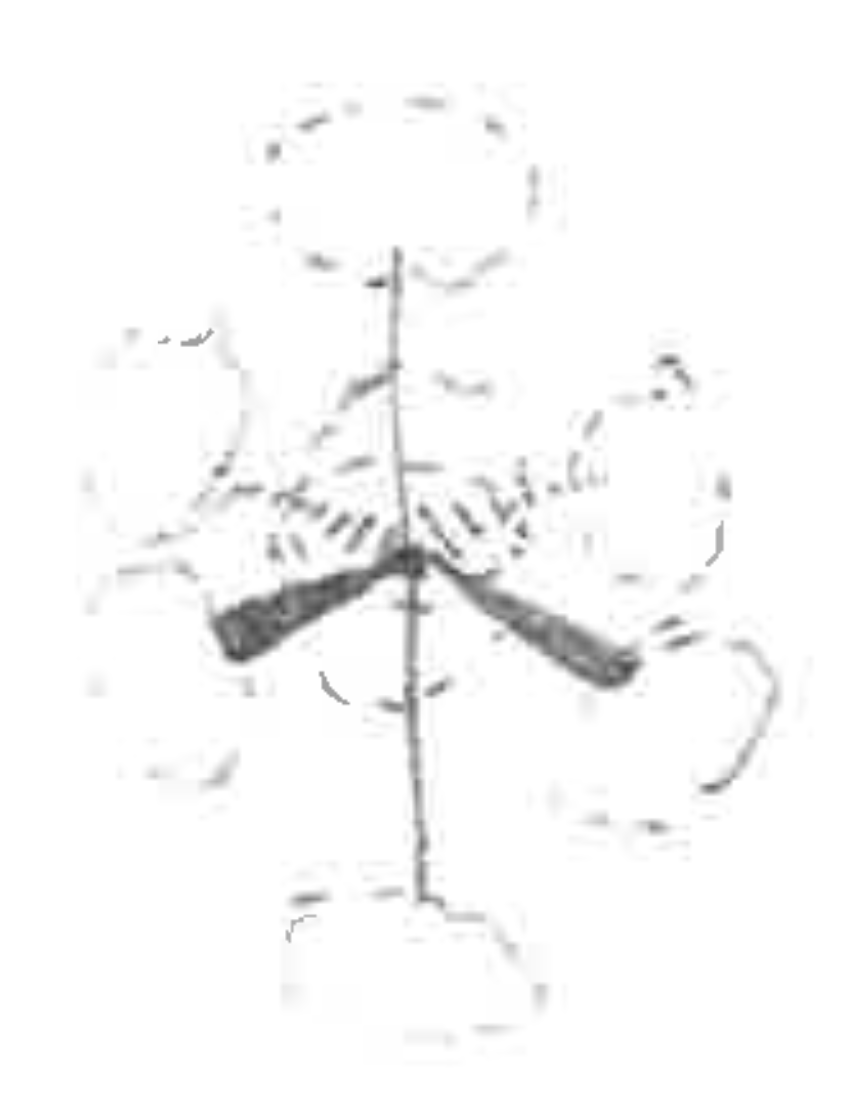
\includegraphics[width=0.7\linewidth]{../ExtFiles/SALC-SF6a.png}
                    \caption{$a_{1g}$.}
                    \label{fig:SALC-SF6a}
                \end{subfigure}
                \begin{subfigure}[b]{0.24\linewidth}
                    \centering
                    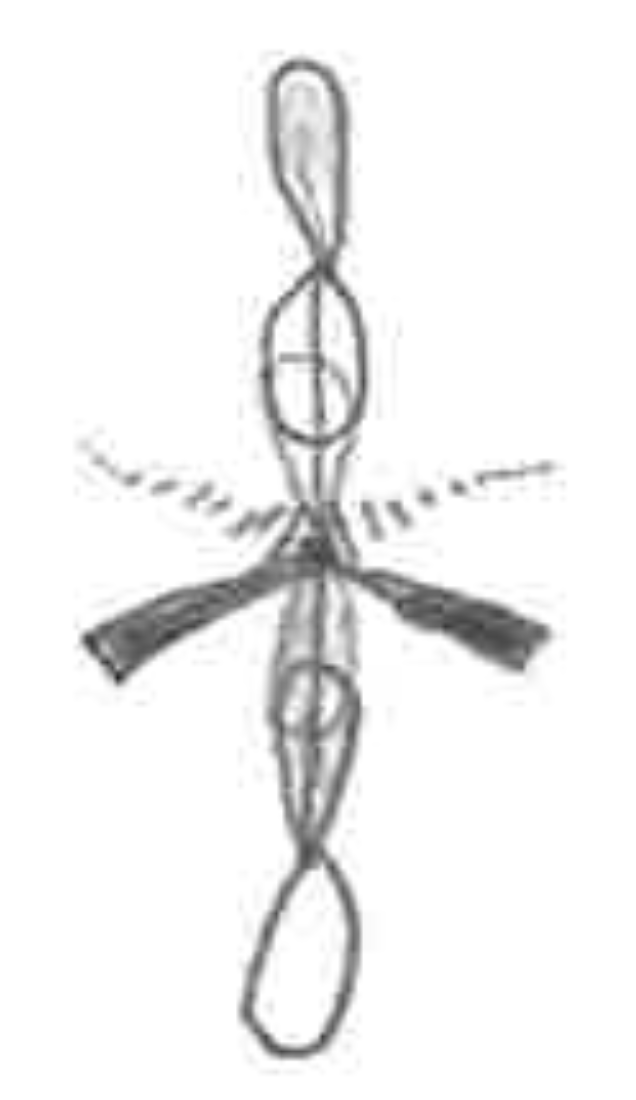
\includegraphics[width=0.5\linewidth]{../ExtFiles/SALC-SF6b.png}
                    \caption{$t_{1u}$.}
                    \label{fig:SALC-SF6b}
                \end{subfigure}
                \begin{subfigure}[b]{0.24\linewidth}
                    \centering
                    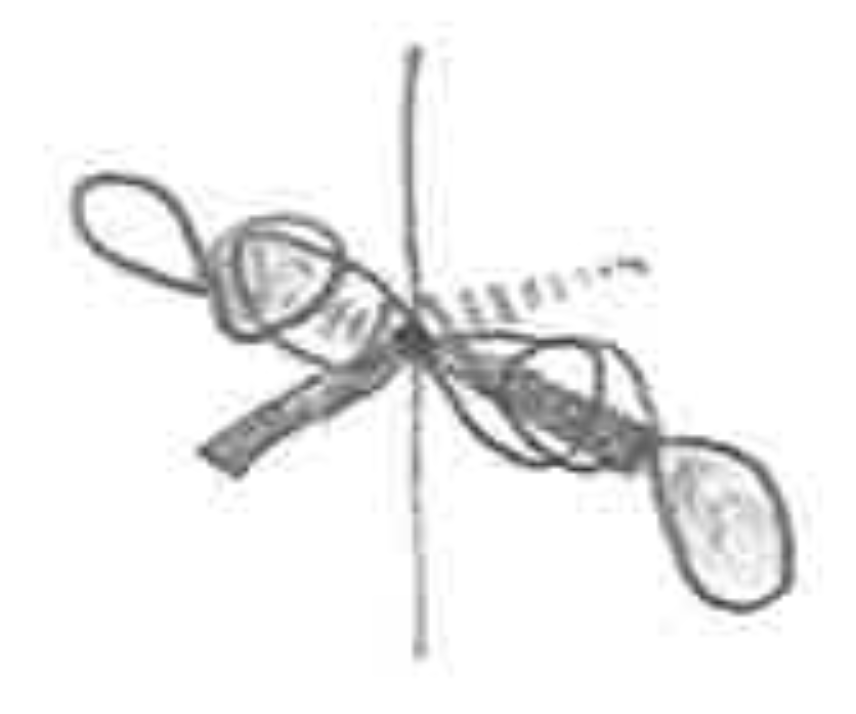
\includegraphics[width=0.8\linewidth]{../ExtFiles/SALC-SF6c.png}
                    \caption{$t_{1u}$.}
                    \label{fig:SALC-SF6c}
                \end{subfigure}
                \begin{subfigure}[b]{0.24\linewidth}
                    \centering
                    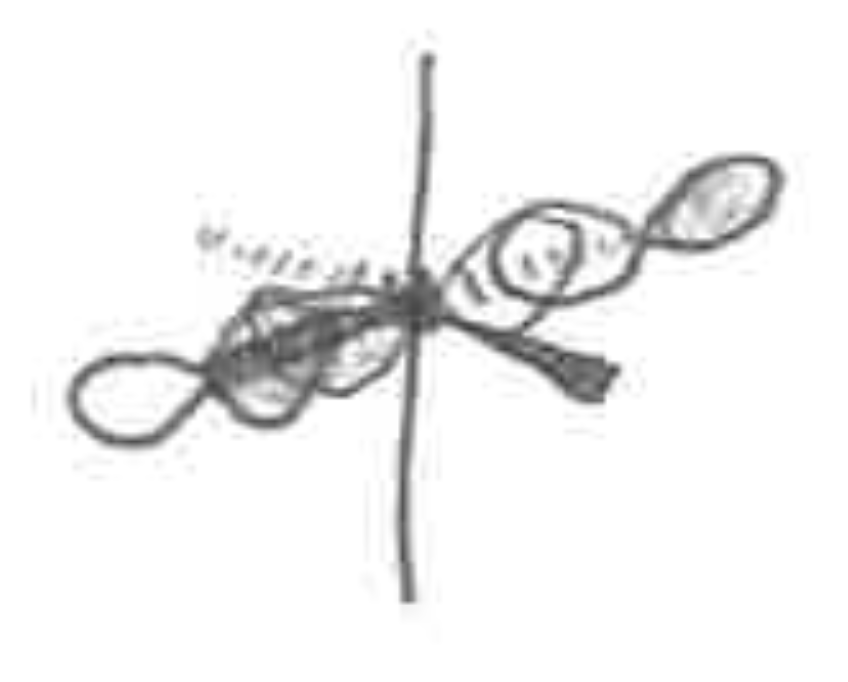
\includegraphics[width=0.8\linewidth]{../ExtFiles/SALC-SF6d.png}
                    \caption{$t_{1u}$.}
                    \label{fig:SALC-SF6d}
                \end{subfigure}
            \end{figure}
            \begin{figure}[H]\ContinuedFloat
                \centering
                \begin{subfigure}[b]{0.4\linewidth}
                    \centering
                    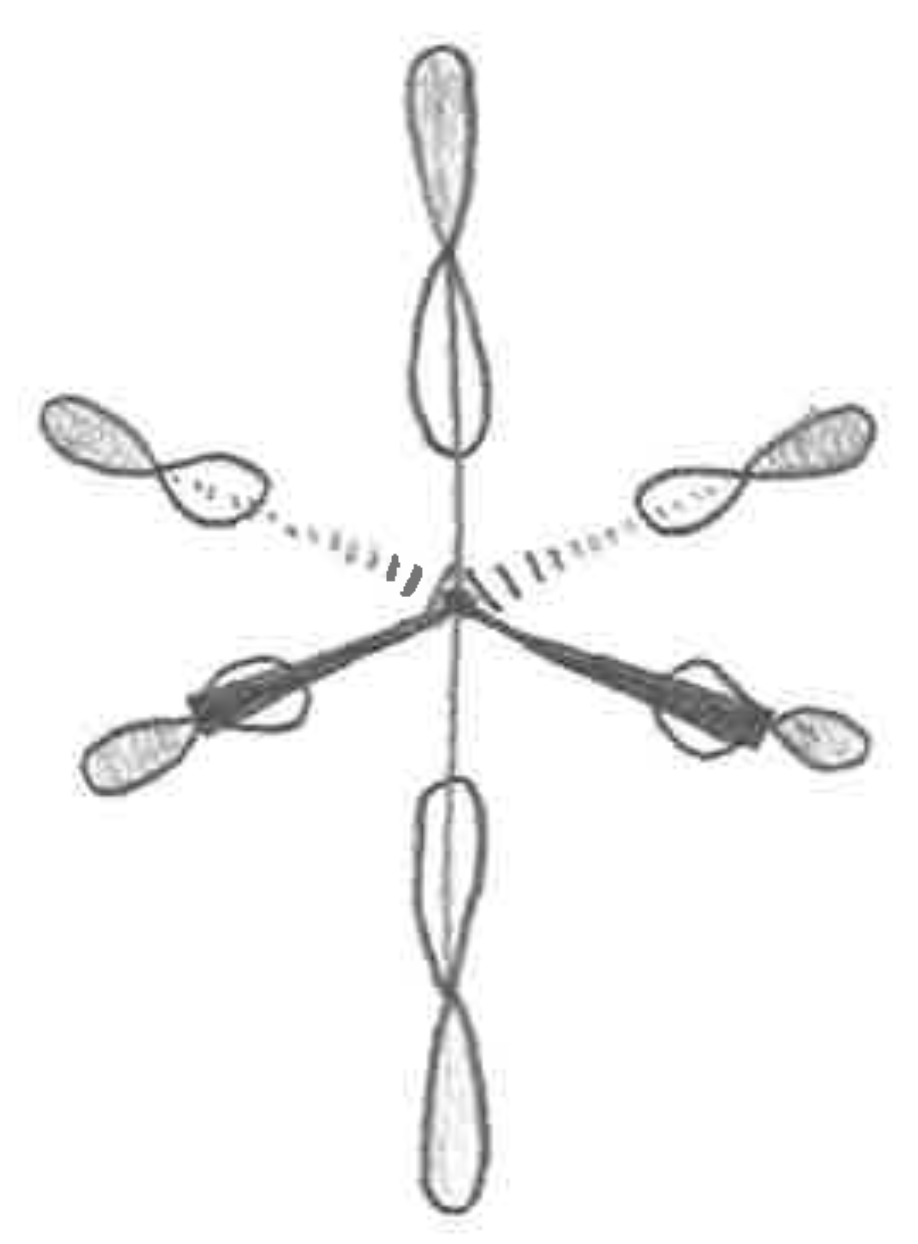
\includegraphics[width=0.7\linewidth]{../ExtFiles/SALC-SF6e.png}
                    \caption{$e_{g}$.}
                    \label{fig:SALC-SF6e}
                \end{subfigure}
                \begin{subfigure}[b]{0.4\linewidth}
                    \centering
                    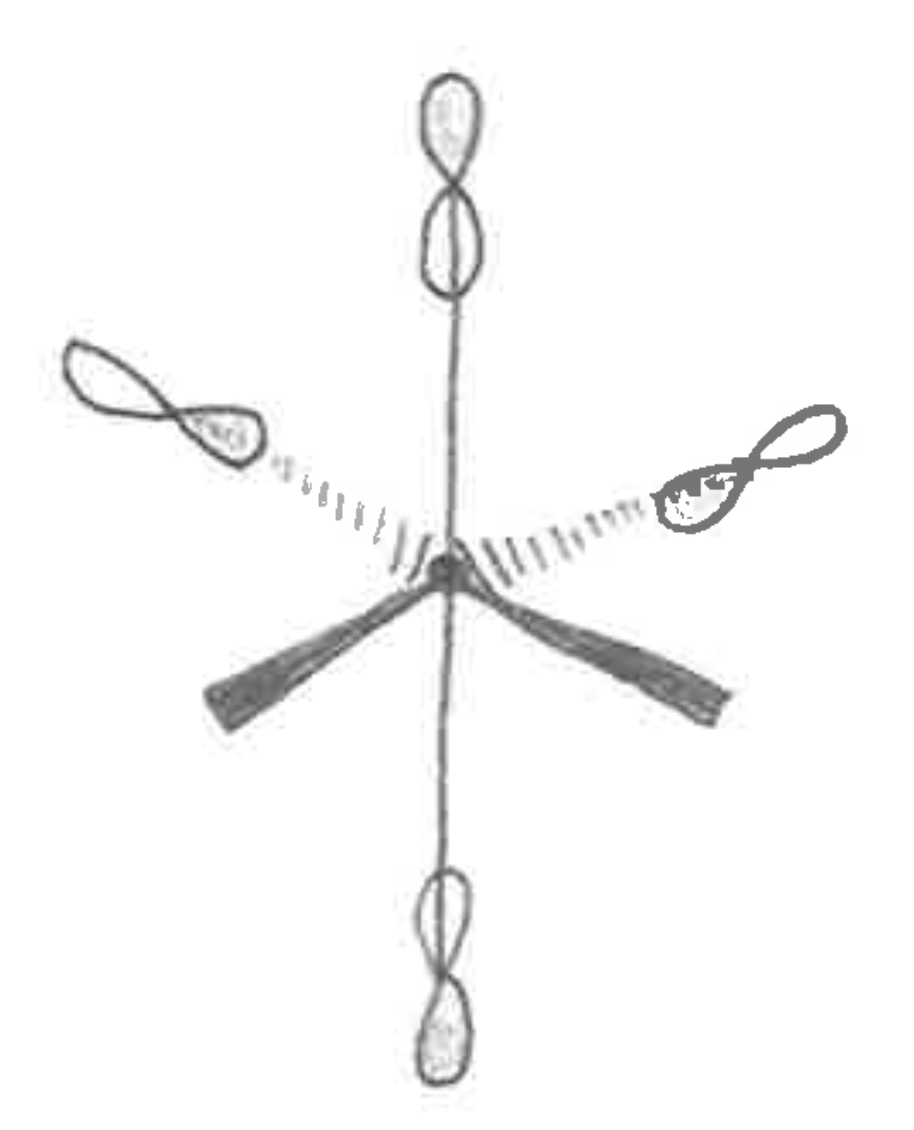
\includegraphics[width=0.7\linewidth]{../ExtFiles/SALC-SF6f.png}
                    \caption{$e_{g}$.}
                    \label{fig:SALC-SF6f}
                \end{subfigure}
                \caption{SALCs for \ce{SF6}.}
                \label{fig:SALC-SF6}
            \end{figure}
        \end{proof}
        \item Label the MO's with the appropriate Mulliken symbols and show the orbital occupancies (i.e., fill in the MO levels with the proper number of electrons).
        \begin{proof}[Answer]
            See Figure \ref{fig:orbitalDiagram-SF6}.
        \end{proof}
        \item Based on the MO diagram, comment on the number of bonding electrons in \ce{SF6} and the bond-order of each \ce{S-F} bond.
        \begin{proof}[Answer]
            There are 8 bonding electrons (the two in the $1a_{1g}$ orbital, and the six in the degenerate $1t_{1u}$ orbitals; the four in the degenerate $1e_g$ orbitals are nonbonding and all anti-bonding orbitals are unfilled). Since the bond order is one half the number of bonding electrons divided by the number of bonds, we have $\text{B.O.}=\frac{2}{3}$.
        \end{proof}
    \end{enumerate}
\end{enumerate}


% Maziotti is a good QMech professor.
% Chem libre texts for sketching MOs.
% Show coefficients.
% Bond order correct.
% Show valence shell IPs in diagram.




\end{document}